\documentclass[10pt]{article}
\usepackage{graphicx,geometry,amssymb,amsmath,amsfonts}
\usepackage{float}
\restylefloat{table}
\usepackage{lscape}
\usepackage{verbatim,latexsym}
\usepackage{Sweave}
\usepackage{epstopdf}
\usepackage{subfigure}
\usepackage{amsthm,graphicx,wasysym}
%\usepackage{titlesec}
\usepackage[utf8]{inputenc}
\usepackage[english]{babel}
\usepackage{longtable}

\usepackage{color}   % May be necessary if you want to color links and for color text
\usepackage[dvipsnames]{xcolor}



\usepackage{hyperref}
\hypersetup{
    colorlinks=true, %set true if you want colored links
    linktoc=all,     %set to all if you want both sections and subsections linked
    linkcolor=blue,  %choose some color if you want links to stand out
}


\setlength{\parindent}{0em}
\setlength{\parskip}{0em}
\renewcommand{\baselinestretch}{1.0}

\geometry{left=1.25in, right=1.25in, top=1in, bottom=1in}

\title{Comparing $C^r$ Values with Network Perturbation Results - Focal Species: Monarch}
\date{}       
\author{Joanna Bieri, Christine Sample, Brady Mattsson, Darius Semmens, and ...}

\begin{document}
\Sconcordance{concordance:MonarchAnalysisReviewJune2018-copy.tex:MonarchAnalysisReviewJune2018-copy.rnw:%
1 50 1 1 12 53 1 1 4 10 0 1 2 1 1 1 39 30 1 1 19 17 1 1 54 33 1 1 54 29 %
1 1 52 35 1 1 53 23 1}


\newcommand{\multilineR}[1]{\begin{tabular}[b]{@{}r@{}}#1\end{tabular}}
\newcommand{\multilineL}[1]{\begin{tabular}[b]{@{}l@{}}#1\end{tabular}}
\newcommand{\multilineC}[1]{\begin{tabular}[b]{@{}c@{}}#1\end{tabular}}

\thispagestyle{empty}

\maketitle

\tableofcontents


\section{Monarch Notes and Generalized \texorpdfstring{$C^r$}{CR} }
We model a population of Monarch Butterfly building our model based on the formulation in  {\it{A general modeling framework for describing spatially structured population dynamics}} by Sample et. al.

We track the population at four nodes: node 1 (Nonbreeding Only - winter), node 2 (Breeding Only - April/May/September), node 3 (Breeding Only - May-Sep), node 4 (Breeding Only - June/July/August). The population is modeled through seven times steps each season:
\begin{itemize}
\item Winter, all migrants start in the nonbreeding only node. Survival of adults is constant at 0.939. 
\item April, all migrants are in breeding node 2. Survival of adults is constant at 0.308.
\item May, all migrants are in breeding nodes 2 \& 3. Survival of adults is constant at 0.308.
\item June, July, and August, all migrants are in breeding nodes 3 \& 4. Survival of adults is constant at 0.308.
\item September, all migrants are in breeding nodes 2 \& 3. Survival of adults is constant at 0.308.
\end{itemize}

We use a generalized network model formulation were we define one time step as

\begin{equation}
\vec{\mathbf{N}}_{t+1}={\mathbf{A}_t}\vec{\mathbf{N}}_t
\end{equation}

Where $\vec{\mathbf{N}}_{t}$ contains the population at each of the $n$ nodes and $c$ classes at time $t$. The matrix $\mathbf{A}_t$ contains all of the demographic node update and migration data for time $t$. (Christine and Joanna have a draft of a paper with this construction).


Within the monarch code we calculate the $C^r$ values for both the origin and the intermediate nodes during each season. We use a generalized one equation definition of $C^r$ in matrix form. %{\it{This generalized version is from Joanna and Christine and has not yet been published, currently in draft form. It allows for complete generality in the number of nodes, classes, and seasons.}}

\begin{equation}
\vec{\mathbf{C}}_t=\left(\prod_{\tau=t}^{t+s-1}\mathbf{A}_\tau^T\right)\vec{\mathbf{1}}_{nc}
\end{equation}

where $s$ is the total number of seasons in one anual cycle, for the monarchs $s=7$ and $\vec{\mathbf{C}}_t$ is a column vector that contains the $C^r$ values at each node for each class for focal season, or time, $t$. 

We note that because the code is run to equillibrium, the overall growth rate of the nework is equal to one. We can calculate the growth rate using:

\begin{equation}
\lambda_t= \frac{\vec{\mathbf{N}}_t^T}{N_t^{tot}}\vec{\mathbf{C}}_t
\label{lambda}
\end{equation}\\
where $N_t^{tot}$ is the sum of the equilibrium population values across all nodes and all classes in the network and is represented by the following summation
\begin{equation}
N_t^{tot}=\sum_{r=1}^n\sum_{x=1}^{c}N^x_{r,t}
\end{equation}

\section{Density Dependence in the Monarch Population}
%
For the monarchs, the $f$ function is density dependent and is given by:
\begin{equation}\label{f_update}
f_{i,t}= \underbrace{s_i^A \cdot N_{i,t}}_{\text{adults that survive}} + \underbrace{s_i^A\cdot s_i^P\cdot s_i^L\cdot E\cdot N_{i,t}}_{\text{eggs that survive and transition to adults}}
\end{equation}
%
$s_i^A$ and $s_i^p$ are constant, but $s_i^L$, which represents larval survival, is dependent on egg density per milkweed stem at node $i$.
\section{Baseline Simulation}
% 
The baseline simulation gives us identical results to {\it{A general modeling framework for describing spatially
structured population dynamics}} by Sample et. al. We find that the long term carrying capacity for each node during the nonbreeding season, including all classes, is

\begin{Schunk}
\begin{Soutput}
season 1 : k= 104369867 0 0 0
season 2 : k= 0 50678505 0 0
season 3 : k= 0 45341487 20370029 0
season 4 : k= 0 0 53525729 33199558
season 5 : k= 0 0 45933321 88548303
season 6 : k= 0 0 72219163 70020140
season 7 : k= 0 62180832 66308229 0
\end{Soutput}
\end{Schunk}



\begin{figure}[H]
\begin{center}
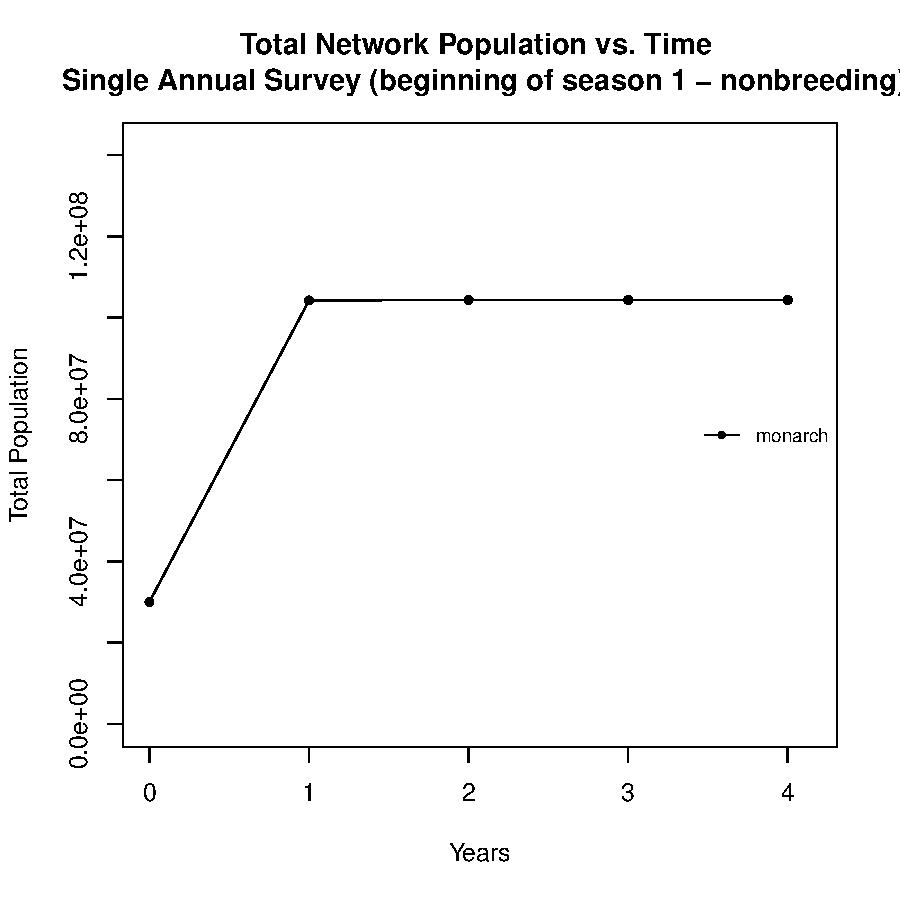
\includegraphics[width=.7\textwidth, height=.6\textwidth]{RGraphics-monarchbaseline}
\caption{Baseline results: population over time at nonbreeding node.}\label{fig:monarchbaseline}
\end{center}
\end{figure}

\clearpage

%%%%%%%%%%%%%%%%%%%%%%%%%%%%%%%%%%%%%%%%%%%%%%%%%%%%%%%%%%%%%%%%%%%
%%%%%%%%%%%%%%%%%%%%%%%%%%%%%%%%%%%%%%%%%%%%%%%%%%%%%%%%%%%%%%%%%%%
%%%%%%%%%%%%%%%%%%%%%%%%%%%%%%%%%%%%%%%%%%%%%%%%%%%%%%%%%%%%%%%%%%%

\section{Perturbation Experiment - Perturbing Node Survival Rates}

To investigate the utility of the metrics as an indicator of the change in carrying capacity $K$ we consider the following perturbations to the survival rate at each node:

\[PERT = .9, .8, .7, .6, .5\]

Some notes about the simulations:
\begin{itemize}
\item All simulations are run to equillibrium with an error tollerance of within 1 animal, meaning the network growth rate $\lambda=1$.
\item We only cary out negative perturbations because positive perturbations will cause survival rates to exceed 1.
\end{itemize}
%  


\newpage 



\section{Monarch Plots - June 2018 - to Match Pintail Outputs}

We will consider metrics for the x-axis of our graph:
\begin{itemize}
\item Baseline $C^r$ vs $K$ perturbations - this is the population weighted $C^r$ value averaged across classes and seasons Figure \ref{fig:monarch_barcr_averageCR}
\item Baseline $W^r$ vs $K$ perturbations - the population proportions averaged across seasons Figure \ref{fig:monarch_barcr_WR}
\item Baseline $D_s$ vs $K$ perturbations - the proportional dependence as defined in Bagstad et al, generalizing to account for juveniles: Figure \ref{fig:monarch_barcr_DS}
\item NEW - Baseline Criticality $KR_i$ vs $K$ perturbations - defined as the network growth rate in the absence of node $i$ using a population weighted average across seasons: Figure \ref{fig:monarch_barcr_KR}. Note that because we are at equilibrium the baseline network growth rate is $\lambda = 1$.
\end{itemize}

\newpage
\subsection{Population weighted average \texorpdfstring{$C^r$}{CR}}

In order to be consistent across case studies we decide to calculate $C^r$ using a population weighted average. The general matrix form of $C^r$ results in a $C^r$ values for each node, class, and season. To combine these into a single full year network wide $C^r$ value we first do a population weighted average by class within each node and then do a population weighted average across seasons. This results in a single $C^r$ values for each node.

The Monarch model has seven seasons (Winter, April, May, June, July, August, Sep) and one class (adult females).


\vspace{-.5cm}
\begin{figure}[H]
\begin{center}
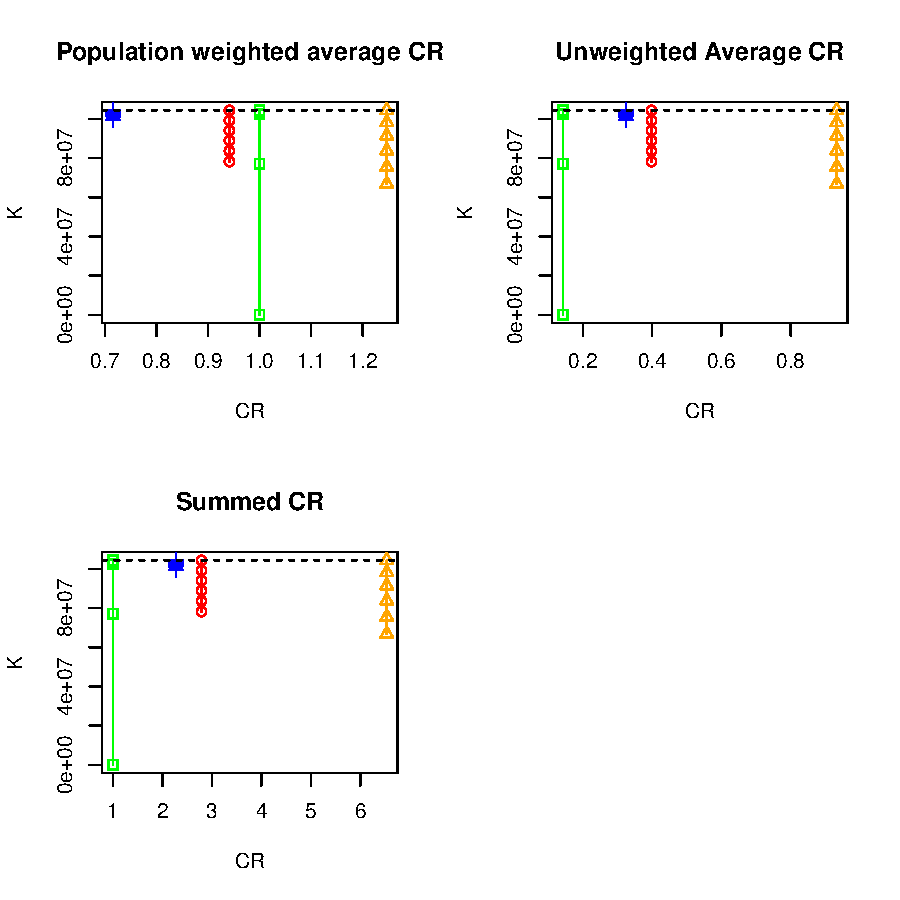
\includegraphics[width=.8\textwidth, height=.8\textwidth]{RGraphics-monarch_barcr_averageCR}
\caption{Perturbation results: Range of K values after perturbations to each node, X-axis represents {\bf{baseline population weighted $C^r$ values}} for each node}\label{fig:monarch_barcr_averageCR}
\end{center}
\end{figure}

\vspace{-.5cm}
\begin{tabular}{|c|c|c|}
\hline
{\color{red} Mexico} & $\Box$ & winter \\
\hline
{\color{orange} South} & $\bigcirc$ & April/May/Sep \\
\hline
{\color{blue} Central} & $\triangle$ &  May/June/July/August/Sep \\
\hline
{\color{green} North} & $+$ & June/July/August \\
\hline
\end{tabular}








\newpage
\subsection{Population Distribution \texorpdfstring{$W^r$}{WR}}

$W^r$ is calculated as the percent of the total population residing at a node. This calculation results in $W^r$ values for each node during each seaons. To get a consistent value for the network, we average (not weighted) across the seasons. The final numbers should sum to one.


\vspace{-.5cm}
\begin{figure}[H]
\begin{center}
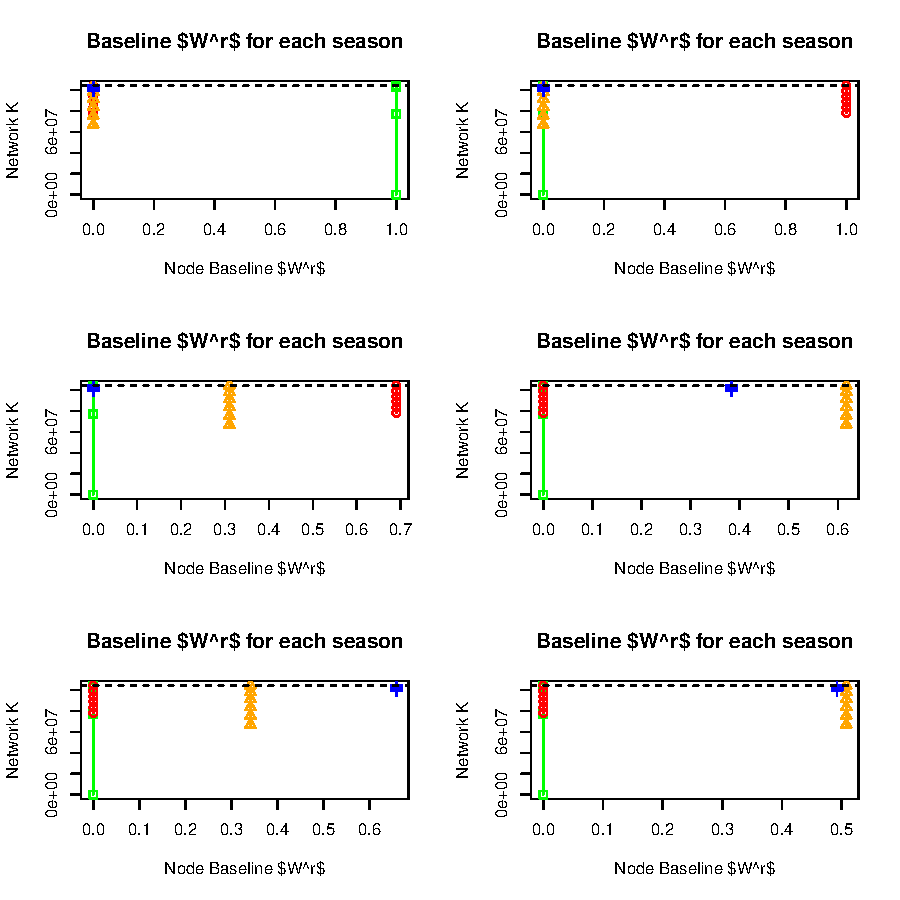
\includegraphics[width=.8\textwidth, height=.8\textwidth]{RGraphics-monarch_barcr_WR}
\caption{Perturbation results: Range of K values after perturbations to each node, X-axis represents baseline average $W^r$ value for each node}\label{fig:monarch_barcr_WR}
\end{center}
\end{figure}

\vspace{-.5cm}
\begin{tabular}{|c|c|c|}
\hline
{\color{red} Mexico} & $\Box$ & winter \\
\hline
{\color{orange} South} & $\bigcirc$ & April/May/Sep \\
\hline
{\color{blue} Central} & $\triangle$ &  May/June/July/August/Sep \\
\hline
{\color{green} North} & $+$ & June/July/August \\
\hline
\end{tabular}




\newpage
\subsection{Proportional Dependence \texorpdfstring{$D_s$}{DS}}

$D_s$ is calculated following Bagstad et al. We first find the population weighted $C^r$ values for each of the seasons and then average across the anual cycle.


\vspace{-.5cm}
\begin{figure}[H]
\begin{center}
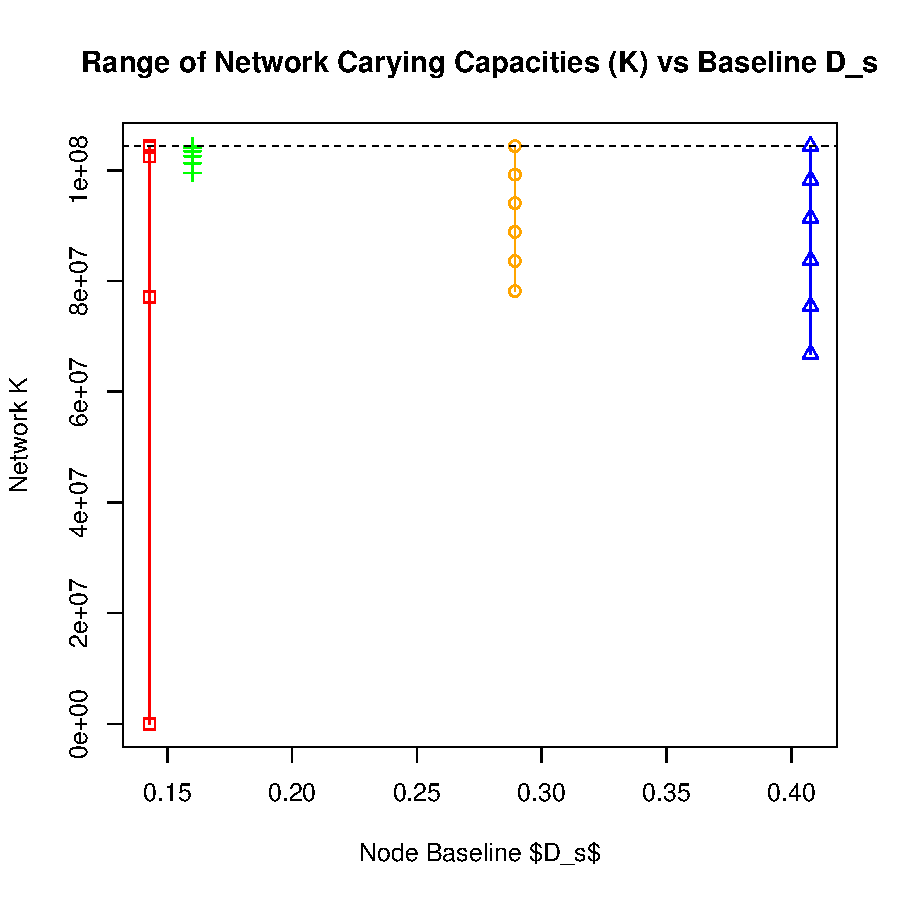
\includegraphics[width=.8\textwidth, height=.8\textwidth]{RGraphics-monarch_barcr_DS}
\caption{Perturbation results: Range of K values after perturbations to each node, X-axis represents baseline $D_s$ value for each node}\label{fig:monarch_barcr_DS}
\end{center}
\end{figure}

\vspace{-.5cm}
\begin{tabular}{|c|c|c|}
\hline
{\color{red} Mexico} & $\Box$ & winter \\
\hline
{\color{orange} South} & $\bigcirc$ & April/May/Sep \\
\hline
{\color{blue} Central} & $\triangle$ &  May/June/July/August/Sep \\
\hline
{\color{green} North} & $+$ & June/July/August \\
\hline
\end{tabular}





\newpage
\subsection{Criticality - NEW \texorpdfstring{$K^r$}{KR}}

Criticality $K^r$ is a new metric concieved of by Christine and her colleagues. The basic idea is that from $C^r$ we can calculate the network growth rate $\lambda$. In the case of a population in equilibrium, like our simulations, $\lambda = 1$. Then one could also calculate a theoretical $C^r$ value as if on of the nodes was removed. From this theoretical $C^r$ value we could calulcate a new network growth rate $\gamma$. We define criticality as 
\[K^r = \lambda - \gamma \]
In other words $K^r$ represents the amount of the network growth rate that flows through the focal node $r$. In our equilibrium case is $K^r=1$ then all of the network growth rate must flow through $r$ and removal of $r$ reduces the new growth rate $\gamma$ to zero. Alternatively, if $K^r=0$ then none of the original network growth rate flows through $r$ and removal of $r$ does not change the growth rate, $\lambda=\gamma=1$.

The $K^r$ calculation results in criticality vales for each node during each season. To get a single yearly value we use a population weighted average.



\vspace{-.5cm}
\begin{figure}[H]
\begin{center}
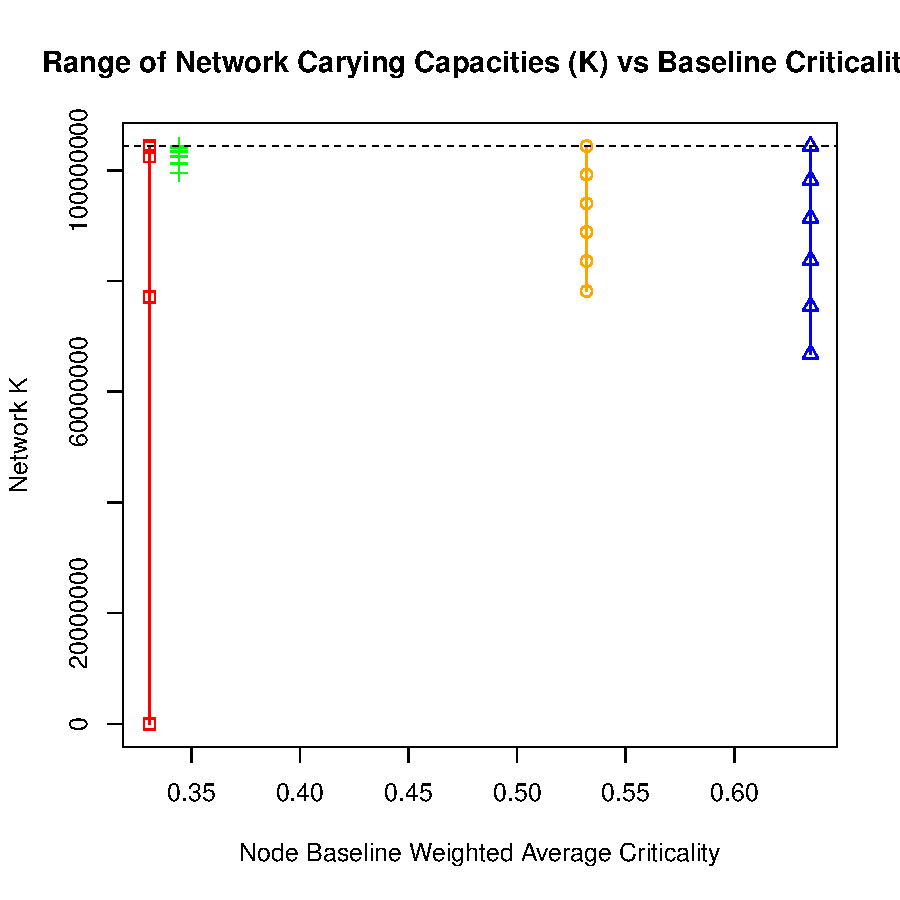
\includegraphics[width=.8\textwidth, height=.8\textwidth]{RGraphics-monarch_barcr_KR}
\caption{Perturbation results: Range of K values after perturbations to each node, X-axis represents baseline Criticality value for each node}\label{fig:monarch_barcr_KR}
\end{center}
\end{figure}

\vspace{-.5cm}
\begin{tabular}{|c|c|c|}
\hline
{\color{red} Mexico} & $\Box$ & winter \\
\hline
{\color{orange} South} & $\bigcirc$ & April/May/Sep \\
\hline
{\color{blue} Central} & $\triangle$ &  May/June/July/August/Sep \\
\hline
{\color{green} North} & $+$ & June/July/August \\
\hline
\end{tabular}


\end{document}
